\part{Differential Geometry}

\chapter{Smooth Manifolds}

\section{Topological Manifolds}

\begin{definition}[Topological Manifold]
    A \textbf{topological manifold} of dimension $n$ is a topological space $M$ satisfying:
    \begin{enumerate}
        \item $M$ is Hausdorff: for any two distinct points $p, q \in M$, there exist disjoint open sets $U, V$ with $p \in U$ and $q \in V$.
        \item $M$ is second countable: there exists a countable basis for the topology.
        \item $M$ is locally Euclidean of dimension $n$: every point $p \in M$ has a neighborhood homeomorphic to an open subset of $\mathbb{R}^n$.
    \end{enumerate}
\end{definition}

\begin{definition}[Chart]
    A \textbf{chart} (or \textbf{coordinate chart}) on $M$ is a pair $(U, \varphi)$ where $U \subseteq M$ is open and $\varphi: U \to \varphi(U) \subseteq \mathbb{R}^n$ is a homeomorphism onto an open subset of $\mathbb{R}^n$. We call $U$ a \textbf{coordinate domain} and $\varphi$ a \textbf{coordinate map}.

    If $\varphi(p) = (x^1, \ldots, x^n)$, we call $(x^1, \ldots, x^n)$ the \textbf{local coordinates} of $p$ in this chart.
\end{definition}

\begin{center}
    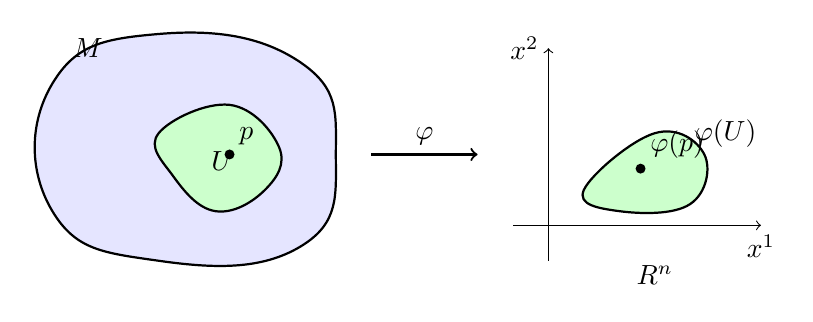
\begin{tikzpicture}[scale=0.9]
        % Manifold M (curved surface)
        \draw[thick, fill=blue!10] plot[smooth cycle, tension=0.8] coordinates {(-2,1.5) (-0.5,2.2) (1.5,1.8) (2,0.5) (1.5,-0.8) (-0.5,-1) (-2,-0.3)};
        \node at (-1.5,2) {$M$};

        % Region U on manifold
        \draw[thick, fill=green!20] plot[smooth cycle, tension=0.7] coordinates {(-0.5,0.8) (0.5,1.2) (1.2,0.6) (1,0) (0.3,-0.3) (-0.3,0.2)};
        \node at (0.4,0.4) {$U$};

        % Point p
        \fill (0.5,0.5) circle (2pt);
        \node[above right] at (0.5,0.5) {$p$};

        % Arrow for phi
        \draw[->, thick] (2.5,0.5) -- (4,0.5);
        \node[above] at (3.25,0.5) {$\varphi$};

        % R^n (coordinate plane)
        \draw[->] (5,-1) -- (5,2) node[left] {$x^2$};
        \draw[->] (4.5,-0.5) -- (8,-0.5) node[below] {$x^1$};

        % phi(U) region
        \draw[thick, fill=green!20] plot[smooth cycle, tension=0.7] coordinates {(5.5,0) (6.5,0.8) (7.2,0.5) (7,-0.2) (6,-0.3)};
        \node at (7.5,0.8) {$\varphi(U)$};

        % Point phi(p)
        \fill (6.3,0.3) circle (2pt);
        \node[above right] at (6.3,0.3) {$\varphi(p)$};

        \node at (6.5,-1.2) {$\mathbb{R}^n$};
    \end{tikzpicture}
\end{center}

\begin{definition}[Transition Map]
    Given two charts $(U, \varphi)$ and $(V, \psi)$ with $U \cap V \neq \emptyset$, the \textbf{transition map} is:
    \[
        \psi \circ \varphi^{-1}: \varphi(U \cap V) \to \psi(U \cap V)
    \]
    This is a homeomorphism between open subsets of $\mathbb{R}^n$.
\end{definition}

\begin{center}
    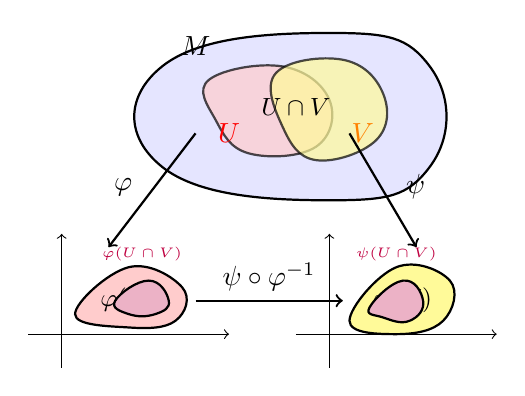
\begin{tikzpicture}[scale=0.85]
        % Manifold M at top
        \draw[thick, fill=blue!10] plot[smooth cycle, tension=0.8] coordinates {(-1.5,4) (1,4.5) (2.5,4) (2.5,2.5) (1,2) (-1.5,2.5)};
        \node at (-1,4.3) {$M$};

        % U region
        \draw[thick, fill=red!20, opacity=0.7] plot[smooth cycle, tension=0.7] coordinates {(-0.8,3.8) (0.3,4) (1,3.5) (0.8,2.8) (-0.2,2.7) (-0.7,3.2)};
        \node[red] at (-0.5,3) {$U$};

        % V region
        \draw[thick, fill=yellow!40, opacity=0.7] plot[smooth cycle, tension=0.7] coordinates {(0.2,3.9) (1.2,4.1) (1.8,3.6) (1.7,2.9) (0.8,2.6) (0.3,3.1)};
        \node[orange] at (1.5,3) {$V$};

        % U cap V (intersection)
        \node at (0.5,3.4) {\small$U \cap V$};

        % phi(U) bottom left
        \draw[->] (-3,-0.5) -- (-3,1.5);
        \draw[->] (-3.5,0) -- (-0.5,0);
        \draw[thick, fill=red!20] plot[smooth cycle, tension=0.7] coordinates {(-2.8,0.3) (-2,1) (-1.2,0.7) (-1.3,0.2) (-2,0.1)};
        \node at (-2,0.5) {\small$\varphi(U)$};
        \draw[thick, fill=purple!30] plot[smooth cycle, tension=0.8] coordinates {(-2.2,0.5) (-1.7,0.8) (-1.4,0.5) (-1.6,0.3) (-2,0.3)};

        % psi(V) bottom right
        \draw[->] (1,-0.5) -- (1,1.5);
        \draw[->] (0.5,0) -- (3.5,0);
        \draw[thick, fill=yellow!40] plot[smooth cycle, tension=0.7] coordinates {(1.3,0.2) (2,1) (2.8,0.8) (2.7,0.2) (2,0)};
        \node at (2.1,0.5) {\small$\psi(V)$};
        \draw[thick, fill=purple!30] plot[smooth cycle, tension=0.8] coordinates {(1.6,0.4) (2.1,0.8) (2.4,0.5) (2.2,0.2) (1.8,0.25)};

        % Arrows
        \draw[->, thick] (-1,3) -- (-2.3,1.3);
        \node[left] at (-1.8,2.2) {$\varphi$};

        \draw[->, thick] (1.3,3) -- (2.3,1.3);
        \node[right] at (2,2.2) {$\psi$};

        \draw[->, thick] (-1,0.5) -- (1.2,0.5);
        \node[above] at (0.1,0.5) {$\psi \circ \varphi^{-1}$};

        % Labels for intersection images
        \node[purple] at (-1.8,1.2) {\tiny$\varphi(U \cap V)$};
        \node[purple] at (2,1.2) {\tiny$\psi(U \cap V)$};
    \end{tikzpicture}
\end{center}

\section{Smooth Structures}

\begin{definition}[Smoothly Compatible Charts]
    Two charts $(U, \varphi)$ and $(V, \psi)$ are \textbf{smoothly compatible} if either $U \cap V = \emptyset$, or the transition map $\psi \circ \varphi^{-1}$ is a smooth (i.e., $C^\infty$) diffeomorphism.
\end{definition}

\begin{definition}[Smooth Atlas]
    A \textbf{smooth atlas} on $M$ is a collection $\mathcal{A} = \{(U_\alpha, \varphi_\alpha)\}_{\alpha \in A}$ of charts such that:
    \begin{enumerate}
        \item The coordinate domains cover $M$: $\bigcup_{\alpha \in A} U_\alpha = M$.
        \item Any two charts in $\mathcal{A}$ are smoothly compatible.
    \end{enumerate}
\end{definition}

\begin{definition}[Maximal Atlas / Smooth Structure]
    A smooth atlas $\mathcal{A}$ is \textbf{maximal} if it is not properly contained in any larger smooth atlas. A \textbf{smooth structure} on $M$ is a maximal smooth atlas.

    A \textbf{smooth manifold} is a topological manifold equipped with a smooth structure.
\end{definition}

\begin{proposition}
    Every smooth atlas $\mathcal{A}$ is contained in a unique maximal atlas, consisting of all charts smoothly compatible with every chart in $\mathcal{A}$.
\end{proposition}

\begin{example}[Standard Smooth Structure on $\mathbb{R}^n$]
    $\mathbb{R}^n$ with the single chart $(\mathbb{R}^n, \mathrm{id})$ defines a smooth structure. This is the \textbf{standard smooth structure}.
\end{example}

\begin{example}[The $n$-Sphere $S^n$]
    $S^n = \{x \in \mathbb{R}^{n+1} : |x| = 1\}$ is a smooth $n$-manifold. One atlas consists of stereographic projections from the north and south poles:
    \begin{align*}
        \sigma_N: S^n \setminus \{N\} & \to \mathbb{R}^n, \quad (x^1, \ldots, x^{n+1}) \mapsto \frac{1}{1 - x^{n+1}}(x^1, \ldots, x^n) \\
        \sigma_S: S^n \setminus \{S\} & \to \mathbb{R}^n, \quad (x^1, \ldots, x^{n+1}) \mapsto \frac{1}{1 + x^{n+1}}(x^1, \ldots, x^n)
    \end{align*}
    The transition map $\sigma_S \circ \sigma_N^{-1}(y) = y/|y|^2$ is smooth on $\mathbb{R}^n \setminus \{0\}$.
\end{example}

\begin{center}
    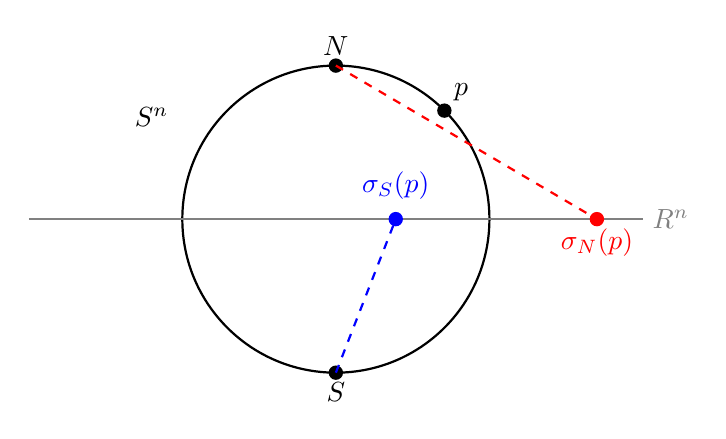
\begin{tikzpicture}[scale=1.3]
        % Circle (S^1 cross-section)
        \draw[thick] (0,0) circle (1.5);

        % Horizontal plane (equator extended)
        \draw[thick, gray] (-3,0) -- (3,0);
        \node[gray, right] at (3,0) {$\mathbb{R}^n$};

        % North and South poles
        \fill (0,1.5) circle (2pt);
        \node[above] at (0,1.5) {$N$};
        \fill (0,-1.5) circle (2pt);
        \node[below] at (0,-1.5) {$S$};

        % Point P on circle
        \fill (1.06,1.06) circle (2pt);
        \node[above right] at (1.06,1.06) {$p$};

        % Stereographic projection from N
        \draw[thick, red, dashed] (0,1.5) -- (2.55,0);
        \fill[red] (2.55,0) circle (2pt);
        \node[red, below] at (2.55,0) {$\sigma_N(p)$};

        % Stereographic projection from S
        \draw[thick, blue, dashed] (0,-1.5) -- (0.585,0);
        \fill[blue] (0.585,0) circle (2pt);
        \node[blue, above] at (0.585,0.1) {$\sigma_S(p)$};

        % Labels
        \node at (-1.8,1) {$S^n$};
    \end{tikzpicture}
\end{center}

\section{Smooth Maps}

\begin{definition}[Smooth Function]
    Let $M$ be a smooth manifold. A function $f: M \to \mathbb{R}$ is \textbf{smooth} if for every chart $(U, \varphi)$, the composition $f \circ \varphi^{-1}: \varphi(U) \to \mathbb{R}$ is smooth in the usual sense.

    We write $C^\infty(M)$ for the set of all smooth real-valued functions on $M$.
\end{definition}

\begin{definition}[Smooth Map Between Manifolds]
    Let $M$ and $N$ be smooth manifolds. A continuous map $F: M \to N$ is \textbf{smooth} if for every $p \in M$, there exist charts $(U, \varphi)$ around $p$ and $(V, \psi)$ around $F(p)$ such that $\psi \circ F \circ \varphi^{-1}$ is smooth.
\end{definition}

\begin{definition}[Diffeomorphism]
    A smooth map $F: M \to N$ is a \textbf{diffeomorphism} if it is bijective and $F^{-1}$ is also smooth. If such an $F$ exists, $M$ and $N$ are \textbf{diffeomorphic}.
\end{definition}

\begin{remark}
    $C^\infty(M)$ forms a commutative $\mathbb{R}$-algebra under pointwise operations.
\end{remark}

\chapter{Tangent Spaces}

\section{Derivations and Tangent Vectors}

The key insight is that tangent vectors can be characterized algebraically as derivations on smooth functions, without reference to ambient space.

\begin{definition}[Derivation at a Point]
    Let $M$ be a smooth manifold and $p \in M$. A \textbf{derivation at $p$} is a linear map $v: C^\infty(M) \to \mathbb{R}$ satisfying the \textbf{Leibniz rule}:
    \[
        v(fg) = f(p) \cdot v(g) + g(p) \cdot v(f)
    \]
    for all $f, g \in C^\infty(M)$.
\end{definition}

\begin{definition}[Tangent Space]
    The \textbf{tangent space} to $M$ at $p$, denoted $T_pM$, is the set of all derivations at $p$. This is a real vector space under:
    \[
        (v + w)(f) = v(f) + w(f), \quad (\lambda v)(f) = \lambda \cdot v(f)
    \]
\end{definition}

\begin{center}
    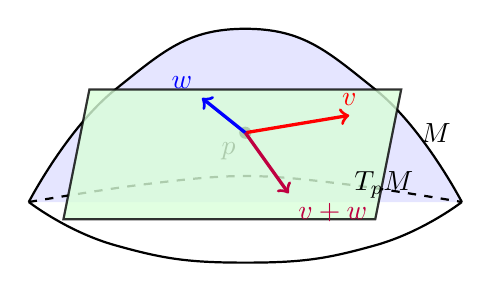
\begin{tikzpicture}[scale=1.1]
        % Draw the surface (paraboloid-like)
        \draw[thick, fill=blue!10] plot[smooth, tension=0.8] coordinates {(-2.5,-0.5) (-1.5,0.8) (0,1.5) (1.5,0.8) (2.5,-0.5)};
        \draw[thick] plot[smooth, tension=0.8] coordinates {(-2.5,-0.5) (-1.5,-1) (0,-1.2) (1.5,-1) (2.5,-0.5)};
        \draw[thick, dashed] plot[smooth, tension=0.6] coordinates {(-2.5,-0.5) (-1.2,-0.3) (0,-0.2) (1.2,-0.3) (2.5,-0.5)};
        \node at (2.2,0.3) {$M$};

        % Point p on surface
        \fill (0,0.3) circle (2pt);
        \node[below left] at (0,0.3) {$p$};

        % Tangent plane (tilted rectangle)
        \draw[thick, fill=green!15, opacity=0.8] (-1.8,0.8) -- (1.8,0.8) -- (1.5,-0.7) -- (-2.1,-0.7) -- cycle;
        \node at (1.6,-0.3) {$T_pM$};

        % Tangent vectors
        \draw[->, very thick, red] (0,0.3) -- (1.2,0.5);
        \node[red, above] at (1.2,0.5) {$v$};

        \draw[->, very thick, blue] (0,0.3) -- (-0.5,0.7);
        \node[blue, above left] at (-0.5,0.7) {$w$};

        \draw[->, very thick, purple] (0,0.3) -- (0.5,-0.4);
        \node[purple, below right] at (0.5,-0.4) {$v + w$};
    \end{tikzpicture}
\end{center}

\begin{lemma}
    If $v \in T_pM$ and $f$ is constant in a neighborhood of $p$, then $v(f) = 0$.
\end{lemma}

\begin{proof}
    If $f \equiv c$ near $p$, write $f = c \cdot 1$ where $1$ is the constant function. Then:
    \[
        v(1) = v(1 \cdot 1) = 1 \cdot v(1) + 1 \cdot v(1) = 2v(1)
    \]
    so $v(1) = 0$. Hence $v(f) = v(c \cdot 1) = c \cdot v(1) = 0$.
\end{proof}

\section{Coordinate Basis}

\begin{definition}[Coordinate Tangent Vectors]
    Let $(U, \varphi)$ be a chart around $p$ with coordinates $(x^1, \ldots, x^n)$. Define the \textbf{coordinate tangent vector} $\left.\frac{\partial}{\partial x^i}\right|_p \in T_pM$ by:
    \[
        \left.\frac{\partial}{\partial x^i}\right|_p (f) = \frac{\partial (f \circ \varphi^{-1})}{\partial r^i}\bigg|_{\varphi(p)}
    \]
    where $r^i$ are the standard coordinates on $\mathbb{R}^n$.
\end{definition}

\begin{theorem}
    Let $M$ be an $n$-dimensional smooth manifold and $(U, \varphi)$ a chart around $p$ with coordinates $(x^1, \ldots, x^n)$. Then $\left\{\left.\frac{\partial}{\partial x^1}\right|_p, \ldots, \left.\frac{\partial}{\partial x^n}\right|_p\right\}$ is a basis for $T_pM$.

    In particular, $\dim T_pM = n$.
\end{theorem}

\begin{corollary}
    Every tangent vector $v \in T_pM$ can be written uniquely as:
    \[
        v = v^i \left.\frac{\partial}{\partial x^i}\right|_p
    \]
    where $v^i = v(x^i)$ and we use Einstein summation convention.
\end{corollary}

\section{The Differential (Pushforward)}

\begin{definition}[Differential of a Smooth Map]
    Let $F: M \to N$ be smooth and $p \in M$. The \textbf{differential} (or \textbf{pushforward}) of $F$ at $p$ is the linear map:
    \[
        dF_p: T_pM \to T_{F(p)}N
    \]
    defined by $(dF_p(v))(g) = v(g \circ F)$ for $v \in T_pM$ and $g \in C^\infty(N)$.
\end{definition}

\begin{center}
    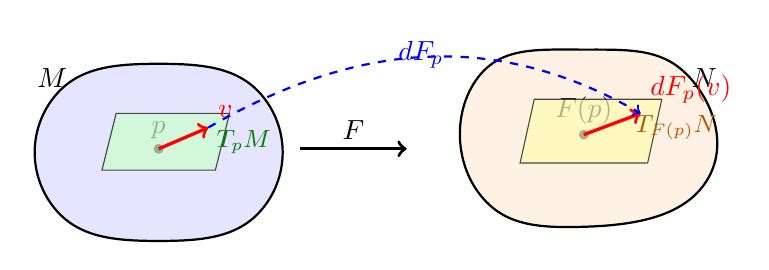
\begin{tikzpicture}[scale=0.9]
        % Manifold M (left)
        \draw[thick, fill=blue!10] plot[smooth cycle, tension=0.8] coordinates {(-4,1.5) (-2.5,2) (-1,1.5) (-1,0) (-2.5,-0.5) (-4,0)};
        \node at (-4,1.8) {$M$};

        % Point p and tangent plane on M
        \fill (-2.5,0.8) circle (2pt);
        \node[above] at (-2.5,0.8) {$p$};

        % Small tangent plane at p
        \draw[fill=green!20, opacity=0.7] (-3.3,0.5) -- (-1.7,0.5) -- (-1.5,1.3) -- (-3.1,1.3) -- cycle;
        \node[green!50!black] at (-1.3,0.9) {\small$T_pM$};

        % Tangent vector v at p
        \draw[->, very thick, red] (-2.5,0.8) -- (-1.8,1.1);
        \node[red, above right] at (-1.8,1.1) {$v$};

        % Arrow F
        \draw[->, very thick] (-0.5,0.8) -- (1,0.8);
        \node[above] at (0.25,0.8) {$F$};

        % Manifold N (right)
        \draw[thick, fill=orange!10] plot[smooth cycle, tension=0.8] coordinates {(2,1.8) (3.5,2.2) (5,1.8) (5.2,0.3) (3.5,-0.3) (2,0.2)};
        \node at (5.2,1.8) {$N$};

        % Point F(p) and tangent plane on N
        \fill (3.5,1) circle (2pt);
        \node[above] at (3.5,1) {$F(p)$};

        % Small tangent plane at F(p)
        \draw[fill=yellow!30, opacity=0.7] (2.6,0.6) -- (4.4,0.6) -- (4.6,1.5) -- (2.8,1.5) -- cycle;
        \node[orange!70!black] at (4.8,1.1) {\small$T_{F(p)}N$};

        % Tangent vector dF(v) at F(p)
        \draw[->, very thick, red] (3.5,1) -- (4.3,1.3);
        \node[red, above right] at (4.3,1.3) {$dF_p(v)$};

        % Curved arrow for dF_p
        \draw[->, thick, dashed, blue] (-1.8,1.1) to[out=30, in=150] (4.3,1.3);
        \node[blue, above] at (1.2,1.8) {$dF_p$};
    \end{tikzpicture}
\end{center}

\begin{remark}
    Other notations for $dF_p$ include $F_{*p}$, $DF_p$, and $T_pF$.
\end{remark}

\begin{proposition}[Chain Rule]
    If $F: M \to N$ and $G: N \to P$ are smooth, then:
    \[
        d(G \circ F)_p = dG_{F(p)} \circ dF_p
    \]
\end{proposition}

\begin{proposition}[Coordinate Expression]
    Let $(U, \varphi)$ be a chart on $M$ with coordinates $(x^i)$ and $(V, \psi)$ a chart on $N$ with coordinates $(y^j)$. If $F: M \to N$ is smooth, then:
    \[
        dF_p\left(\left.\frac{\partial}{\partial x^i}\right|_p\right) = \frac{\partial F^j}{\partial x^i}(p) \left.\frac{\partial}{\partial y^j}\right|_{F(p)}
    \]
    where $F^j = y^j \circ F$ are the component functions.
\end{proposition}

\begin{corollary}
    The matrix of $dF_p$ with respect to coordinate bases is the Jacobian matrix $\left(\frac{\partial F^j}{\partial x^i}\right)$.
\end{corollary}

\chapter{Cotangent Spaces and Differential Forms}

\section{Covectors and the Cotangent Space}

\begin{definition}[Cotangent Space]
    The \textbf{cotangent space} to $M$ at $p$, denoted $T_p^*M$, is the dual vector space to $T_pM$:
    \[
        T_p^*M = (T_pM)^* = \{\omega: T_pM \to \mathbb{R} : \omega \text{ is linear}\}
    \]
    Elements of $T_p^*M$ are called \textbf{covectors} or \textbf{cotangent vectors}.
\end{definition}

\begin{definition}[Differential of a Function]
    For $f \in C^\infty(M)$, the \textbf{differential of $f$ at $p$} is the covector $df_p \in T_p^*M$ defined by:
    \[
        df_p(v) = v(f)
    \]
    for $v \in T_pM$.
\end{definition}

\begin{center}
    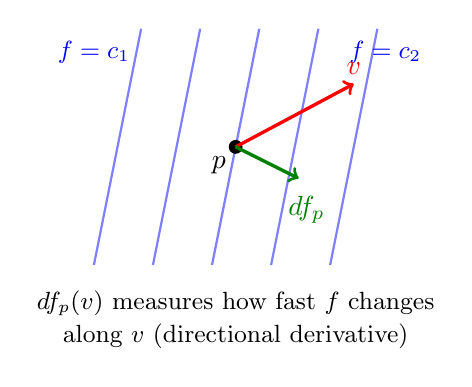
\begin{tikzpicture}[scale=1]
        % Level sets of f
        \foreach \i in {-1.5,-0.75,0,0.75,1.5} {
                \draw[blue!50, thick] plot[smooth, tension=0.8] coordinates {(\i-0.3,-1.5) (\i,0) (\i+0.3,1.5)};
            }

        % Labels for level sets
        \node[blue] at (-1.8,1.2) {\small$f = c_1$};
        \node[blue] at (1.9,1.2) {\small$f = c_2$};

        % Point p
        \fill (0,0) circle (2.5pt);
        \node[below left] at (0,0) {$p$};

        % Tangent vector v
        \draw[->, very thick, red] (0,0) -- (1.5,0.8);
        \node[red, above] at (1.5,0.8) {$v$};

        % df_p shown as stacked planes (covector visualization)
        \draw[->, very thick, green!50!black] (0,0) -- (0.8,-0.4);
        \node[green!50!black, below] at (0.9,-0.5) {$df_p$};

        % Annotation
        \node[align=center] at (0,-2.2) {\small $df_p(v)$ measures how fast $f$ changes\\ \small along $v$ (directional derivative)};
    \end{tikzpicture}
\end{center}

\begin{proposition}[Coordinate Basis for $T_p^*M$]
    If $(x^1, \ldots, x^n)$ are local coordinates near $p$, then $\{dx^1|_p, \ldots, dx^n|_p\}$ is the basis of $T_p^*M$ dual to $\left\{\left.\frac{\partial}{\partial x^1}\right|_p, \ldots, \left.\frac{\partial}{\partial x^n}\right|_p\right\}$:
    \[
        dx^i\left(\frac{\partial}{\partial x^j}\right) = \delta^i_j
    \]
\end{proposition}

\begin{corollary}
    Any covector $\omega \in T_p^*M$ can be written as:
    \[
        \omega = \omega_i \, dx^i|_p
    \]
    where $\omega_i = \omega\left(\frac{\partial}{\partial x^i}\right)$.
\end{corollary}

\begin{proposition}[Differential in Coordinates]
    If $f \in C^\infty(M)$, then in local coordinates:
    \[
        df = \frac{\partial f}{\partial x^i} dx^i
    \]
\end{proposition}

\section{The Pullback}

\begin{definition}[Pullback of a Covector]
    Let $F: M \to N$ be smooth and $p \in M$. The \textbf{pullback} (or \textbf{cotangent map}) is:
    \[
        dF_p^*: T_{F(p)}^*N \to T_p^*M
    \]
    defined by $(dF_p^*\omega)(v) = \omega(dF_p(v))$ for $\omega \in T_{F(p)}^*N$ and $v \in T_pM$.
\end{definition}

\begin{remark}
    Note the reversed direction: while $dF_p$ pushes vectors forward from $M$ to $N$, $dF_p^*$ pulls covectors back from $N$ to $M$.
\end{remark}

\begin{center}
    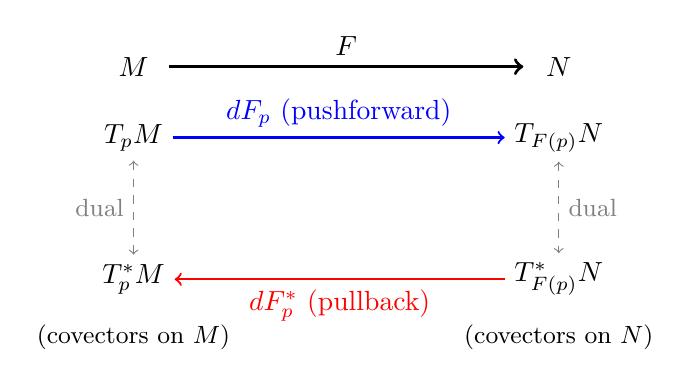
\begin{tikzpicture}[scale=0.9]
        % Left side: M
        \node (TpM) at (0,2) {$T_pM$};
        \node (TpMstar) at (0,0) {$T_p^*M$};
        \node[below] at (0,-0.5) {\small(covectors on $M$)};

        % Right side: N
        \node (TFpN) at (6,2) {$T_{F(p)}N$};
        \node (TFpNstar) at (6,0) {$T_{F(p)}^*N$};
        \node[below] at (6,-0.5) {\small(covectors on $N$)};

        % Horizontal arrows
        \draw[->, thick, blue] (TpM) -- (TFpN) node[midway, above] {$dF_p$ (pushforward)};
        \draw[<-, thick, red] (TpMstar) -- (TFpNstar) node[midway, below] {$dF_p^*$ (pullback)};

        % Vertical pairing arrows
        \draw[<->, dashed, gray] (TpM) -- (TpMstar) node[midway, left] {\small dual};
        \draw[<->, dashed, gray] (TFpN) -- (TFpNstar) node[midway, right] {\small dual};

        % Labels for manifolds
        \node at (0,3) {$M$};
        \node at (6,3) {$N$};

        % F arrow
        \draw[->, very thick] (0.5,3) -- (5.5,3) node[midway, above] {$F$};
    \end{tikzpicture}
\end{center}

\section{Differential 1-Forms}

\begin{definition}[Differential 1-Form]
    A \textbf{differential 1-form} (or simply \textbf{1-form}) on $M$ is a smooth assignment of a covector at each point:
    \[
        \omega: p \mapsto \omega_p \in T_p^*M
    \]
    More precisely, $\omega$ is a smooth section of the cotangent bundle $T^*M$.
\end{definition}

\begin{definition}[Smoothness of 1-Forms]
    A 1-form $\omega$ is \textbf{smooth} if for every smooth vector field $X$, the function $\omega(X): M \to \mathbb{R}$ defined by $p \mapsto \omega_p(X_p)$ is smooth.

    Equivalently, in any local coordinates, if $\omega = \omega_i \, dx^i$, then each coefficient function $\omega_i$ is smooth.
\end{definition}

\begin{definition}[Space of 1-Forms]
    We denote by $\Omega^1(M)$ the $C^\infty(M)$-module of all smooth 1-forms on $M$.
\end{definition}

\begin{example}[The Differential as a 1-Form]
    For any $f \in C^\infty(M)$, its differential $df$ is a smooth 1-form. In coordinates:
    \[
        df = \frac{\partial f}{\partial x^1} dx^1 + \cdots + \frac{\partial f}{\partial x^n} dx^n
    \]
\end{example}

\begin{definition}[Pullback of 1-Forms]
    If $F: M \to N$ is smooth and $\omega \in \Omega^1(N)$, the \textbf{pullback} $F^*\omega \in \Omega^1(M)$ is defined by:
    \[
        (F^*\omega)_p = dF_p^*(\omega_{F(p)})
    \]
    That is, $(F^*\omega)_p(v) = \omega_{F(p)}(dF_p(v))$ for $v \in T_pM$.
\end{definition}

\begin{proposition}
    The pullback satisfies:
    \begin{enumerate}
        \item $F^*(df) = d(f \circ F)$ for $f \in C^\infty(N)$
        \item $(G \circ F)^* = F^* \circ G^*$
        \item $F^*(f\omega) = (f \circ F) \cdot F^*\omega$
    \end{enumerate}
\end{proposition}

\section{Differential $k$-Forms}

\begin{definition}[Multilinear Alternating Maps]
    A map $\omega: (T_pM)^k \to \mathbb{R}$ is:
    \begin{itemize}
        \item \textbf{Multilinear}: linear in each argument
        \item \textbf{Alternating}: $\omega(\ldots, v, \ldots, w, \ldots) = -\omega(\ldots, w, \ldots, v, \ldots)$ when any two arguments are swapped
    \end{itemize}
    We denote the space of such maps by $\Lambda^k(T_p^*M)$.
\end{definition}

\begin{definition}[Differential $k$-Form]
    A \textbf{differential $k$-form} on $M$ is a smooth assignment $\omega: p \mapsto \omega_p \in \Lambda^k(T_p^*M)$.

    We denote the space of smooth $k$-forms by $\Omega^k(M)$.
\end{definition}

\begin{remark}
    Special cases:
    \begin{itemize}
        \item $\Omega^0(M) = C^\infty(M)$ (smooth functions)
        \item $\Omega^1(M)$ = smooth 1-forms (as defined above)
        \item $\Omega^k(M) = \{0\}$ for $k > n = \dim M$
    \end{itemize}
\end{remark}

\section{The Wedge Product}

\begin{definition}[Wedge Product]
    The \textbf{wedge product} (or \textbf{exterior product}) is a bilinear operation:
    \[
        \wedge: \Omega^k(M) \times \Omega^\ell(M) \to \Omega^{k+\ell}(M)
    \]
    For 1-forms $\alpha, \beta$, defined on vectors $v, w$ by:
    \[
        (\alpha \wedge \beta)(v, w) = \alpha(v)\beta(w) - \alpha(w)\beta(v)
    \]
\end{definition}

\begin{center}
    \begin{tikzpicture}[scale=1.2]
        % Origin
        \coordinate (O) at (0,0);

        % Vectors v and w
        \coordinate (V) at (2.5,0.5);
        \coordinate (W) at (1,2);

        % Parallelogram
        \fill[blue!20, opacity=0.7] (O) -- (V) -- ($(V)+(W)$) -- (W) -- cycle;
        \draw[thick, blue] (O) -- (V) -- ($(V)+(W)$) -- (W) -- cycle;

        % Vectors
        \draw[->, very thick, red] (O) -- (V);
        \node[red, below right] at (V) {$v$};

        \draw[->, very thick, green!50!black] (O) -- (W);
        \node[green!50!black, above left] at (W) {$w$};

        % Area label
        \node[blue] at (1.5,1) {$(\alpha \wedge \beta)(v,w)$};

        % Annotation
        \node[align=center] at (1.75,-0.8) {\small Signed area of parallelogram\\ \small spanned by $v$ and $w$};

        % Small orientation arc
        \draw[->, thick] (0.6,0.15) arc (15:60:0.6);
        \node at (0.9,0.6) {\tiny$+$};
    \end{tikzpicture}
\end{center}

\begin{proposition}[Properties of the Wedge Product]
    \begin{enumerate}
        \item \textbf{Associativity}: $(\alpha \wedge \beta) \wedge \gamma = \alpha \wedge (\beta \wedge \gamma)$
        \item \textbf{Graded commutativity}: $\alpha \wedge \beta = (-1)^{k\ell} \beta \wedge \alpha$ for $\alpha \in \Omega^k$, $\beta \in \Omega^\ell$
        \item \textbf{$C^\infty(M)$-linearity}: $(f\alpha) \wedge \beta = f(\alpha \wedge \beta) = \alpha \wedge (f\beta)$
    \end{enumerate}
\end{proposition}

\begin{corollary}
    For any 1-form $\alpha$: $\alpha \wedge \alpha = 0$.
\end{corollary}

\begin{proposition}[Local Expression]
    In local coordinates $(x^1, \ldots, x^n)$, every $k$-form can be written:
    \[
        \omega = \sum_{i_1 < \cdots < i_k} \omega_{i_1 \cdots i_k} \, dx^{i_1} \wedge \cdots \wedge dx^{i_k}
    \]
    where $\omega_{i_1 \cdots i_k} \in C^\infty(M)$.
\end{proposition}

\section{The Exterior Derivative}

\begin{definition}[Exterior Derivative]
    The \textbf{exterior derivative} is the unique family of linear maps:
    \[
        d: \Omega^k(M) \to \Omega^{k+1}(M)
    \]
    satisfying:
    \begin{enumerate}
        \item For $f \in \Omega^0(M) = C^\infty(M)$, $df$ is the differential of $f$
        \item $d^2 = 0$: for any $\omega$, $d(d\omega) = 0$
        \item \textbf{Graded Leibniz rule}: $d(\alpha \wedge \beta) = d\alpha \wedge \beta + (-1)^k \alpha \wedge d\beta$ for $\alpha \in \Omega^k$
    \end{enumerate}
\end{definition}

\begin{center}
    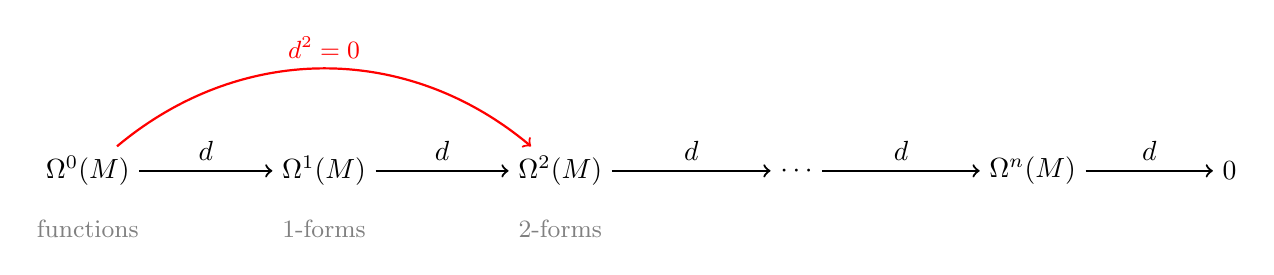
\begin{tikzpicture}[scale=1]
        % de Rham complex
        \node (O0) at (0,0) {$\Omega^0(M)$};
        \node (O1) at (3,0) {$\Omega^1(M)$};
        \node (O2) at (6,0) {$\Omega^2(M)$};
        \node (O3) at (9,0) {$\cdots$};
        \node (On) at (12,0) {$\Omega^n(M)$};
        \node (zero) at (14.5,0) {$0$};

        % Arrows
        \draw[->, thick] (O0) -- (O1) node[midway, above] {$d$};
        \draw[->, thick] (O1) -- (O2) node[midway, above] {$d$};
        \draw[->, thick] (O2) -- (O3) node[midway, above] {$d$};
        \draw[->, thick] (O3) -- (On) node[midway, above] {$d$};
        \draw[->, thick] (On) -- (zero) node[midway, above] {$d$};

        % Labels
        \node[below, gray] at (0,-0.5) {\small functions};
        \node[below, gray] at (3,-0.5) {\small 1-forms};
        \node[below, gray] at (6,-0.5) {\small 2-forms};

        % d^2 = 0 annotation
        \draw[->, thick, red, bend left=40] (O0) to node[above] {\small$d^2 = 0$} (O2);
    \end{tikzpicture}
\end{center}

\begin{proposition}[Coordinate Formula]
    For $\omega = \sum_{I} \omega_I \, dx^I$ where $I = (i_1, \ldots, i_k)$:
    \[
        d\omega = \sum_I d\omega_I \wedge dx^I = \sum_I \frac{\partial \omega_I}{\partial x^j} dx^j \wedge dx^{i_1} \wedge \cdots \wedge dx^{i_k}
    \]
\end{proposition}

\begin{example}
    On $\mathbb{R}^3$ with coordinates $(x, y, z)$:
    \begin{itemize}
        \item If $f \in \Omega^0$: $df = \frac{\partial f}{\partial x}dx + \frac{\partial f}{\partial y}dy + \frac{\partial f}{\partial z}dz$ (gradient)
        \item If $\omega = P\,dx + Q\,dy + R\,dz \in \Omega^1$:
              \[
                  d\omega = \left(\frac{\partial R}{\partial y} - \frac{\partial Q}{\partial z}\right)dy \wedge dz + \left(\frac{\partial P}{\partial z} - \frac{\partial R}{\partial x}\right)dz \wedge dx + \left(\frac{\partial Q}{\partial x} - \frac{\partial P}{\partial y}\right)dx \wedge dy
              \]
              (curl)
    \end{itemize}
\end{example}

\begin{theorem}[Naturality of $d$]
    If $F: M \to N$ is smooth, then $d$ commutes with pullback:
    \[
        F^*(d\omega) = d(F^*\omega)
    \]
    for all $\omega \in \Omega^k(N)$.
\end{theorem}

\begin{definition}[Closed and Exact Forms]
    A $k$-form $\omega$ is:
    \begin{itemize}
        \item \textbf{Closed} if $d\omega = 0$
        \item \textbf{Exact} if $\omega = d\eta$ for some $(k-1)$-form $\eta$
    \end{itemize}
    Since $d^2 = 0$, every exact form is closed. The converse is not always true.
\end{definition}

\begin{center}
    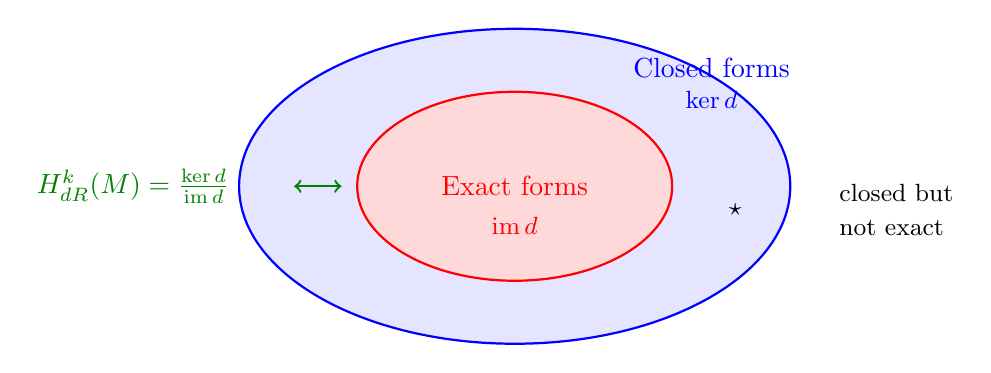
\begin{tikzpicture}[scale=1]
        % Outer ellipse: closed forms
        \draw[thick, blue, fill=blue!10] (0,0) ellipse (3.5 and 2);
        \node[blue] at (2.5,1.5) {Closed forms};
        \node[blue] at (2.5,1.1) {\small$\ker d$};

        % Inner ellipse: exact forms
        \draw[thick, red, fill=red!15] (0,0) ellipse (2 and 1.2);
        \node[red] at (0,0) {Exact forms};
        \node[red] at (0,-0.5) {\small$\mathrm{im}\, d$};

        % H^k annotation
        \draw[<->, thick, green!50!black] (-2.8,0) -- (-2.2,0);
        \node[green!50!black, left] at (-3.5,0) {$H^k_{dR}(M) = \frac{\ker d}{\mathrm{im}\, d}$};

        % Example of closed but not exact
        \node at (2.8,-0.3) {\small$\star$};
        \node[right, align=left] at (4,-0.3) {\small closed but\\ \small not exact};
    \end{tikzpicture}
\end{center}

\begin{definition}[de Rham Cohomology]
    The $k$-th \textbf{de Rham cohomology group} of $M$ is:
    \[
        H^k_{dR}(M) = \frac{\ker(d: \Omega^k \to \Omega^{k+1})}{\mathrm{im}(d: \Omega^{k-1} \to \Omega^k)} = \frac{\{\text{closed } k\text{-forms}\}}{\{\text{exact } k\text{-forms}\}}
    \]
\end{definition}

\begin{theorem}[Poincaré Lemma]
    If $U \subseteq \mathbb{R}^n$ is star-shaped (e.g., convex), then every closed form on $U$ is exact. That is, $H^k_{dR}(U) = 0$ for $k \geq 1$.
\end{theorem}

\chapter{Integration and Stokes' Theorem}

\section{Integration of Differential Forms}

\begin{definition}[Integration of $n$-Forms]
    Let $M$ be an oriented $n$-dimensional manifold and $\omega \in \Omega^n(M)$ a compactly supported $n$-form. In local coordinates where $\omega = f \, dx^1 \wedge \cdots \wedge dx^n$:
    \[
        \int_M \omega = \int_{\mathbb{R}^n} f(x^1, \ldots, x^n) \, dx^1 \cdots dx^n
    \]
    The integral is independent of the choice of positively oriented coordinates.
\end{definition}

\begin{remark}
    The key insight: \textbf{differential forms are the natural objects to integrate}. The wedge product provides the correct transformation law under change of variables (the Jacobian determinant appears automatically).
\end{remark}

\section{Stokes' Theorem}

\begin{theorem}[Generalized Stokes' Theorem]
    Let $M$ be an oriented $n$-dimensional manifold with boundary $\partial M$, and let $\omega \in \Omega^{n-1}(M)$ be a compactly supported $(n-1)$-form. Then:
    \[
        \boxed{\int_M d\omega = \int_{\partial M} \omega}
    \]
\end{theorem}

\begin{center}
    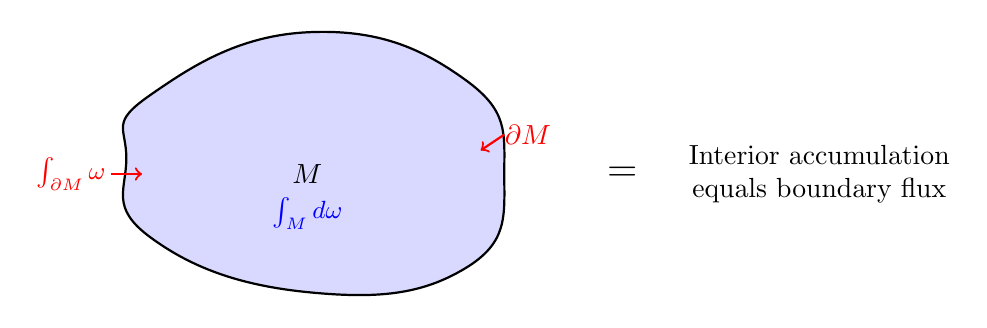
\begin{tikzpicture}[scale=1]
        % Region M
        \draw[thick, fill=blue!15] plot[smooth cycle, tension=0.8] coordinates {(-2,1) (0,1.8) (2,1.2) (2.5,0) (2,-1.2) (0,-1.5) (-2,-0.8) (-2.3,0.2)};
        \node at (0,0) {$M$};
        \node[blue] at (0,-0.5) {\small$\int_M d\omega$};

        % Boundary annotation
        \node[red] at (2.8,0.5) {$\partial M$};
        \draw[->, red, thick] (2.5,0.5) -- (2.2,0.3);

        % Boundary integral annotation
        \node[red] at (-3,0) {\small$\int_{\partial M} \omega$};
        \draw[->, red, thick] (-2.5,0) -- (-2.1,0);

        % Equals sign
        \node at (4,0) {\Large$=$};

        % Right side: conceptual
        \node[align=center] at (6.5,0) {Interior accumulation\\ equals boundary flux};
    \end{tikzpicture}
\end{center}

\begin{remark}
    This single theorem unifies all the classical integration theorems of vector calculus. The exterior derivative $d$ and the boundary operator $\partial$ are \textbf{adjoint} to each other.
\end{remark}

\section{Classical Theorems as Special Cases}

On $\mathbb{R}^3$, we establish correspondences between vector fields and differential forms.

\begin{definition}[Musical Isomorphisms]
    Using the Euclidean metric, we identify:
    \begin{itemize}
        \item Vector field $\mathbf{F} = (P, Q, R)$ with 1-form $\mathbf{F}^\flat = P\,dx + Q\,dy + R\,dz$
        \item Vector field $\mathbf{F}$ with 2-form $\star\mathbf{F}^\flat = P\,dy \wedge dz + Q\,dz \wedge dx + R\,dx \wedge dy$
    \end{itemize}
\end{definition}

\subsection{Gradient, Curl, and Divergence}

The exterior derivative $d$ encodes \textbf{all three} vector calculus differential operators:

\begin{center}
    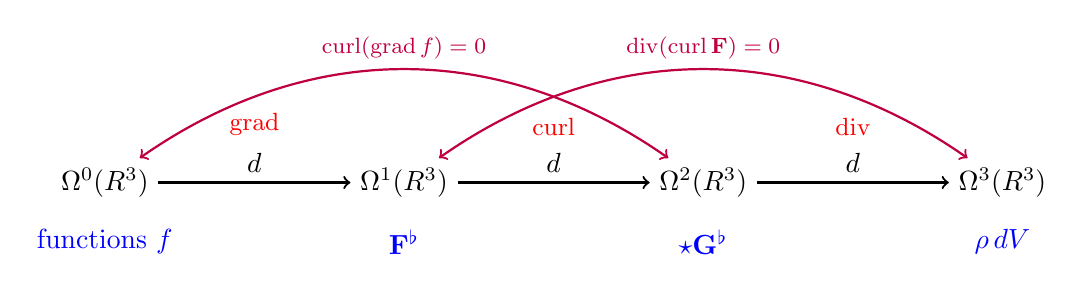
\begin{tikzpicture}[scale=0.95]
        % de Rham complex for R^3
        \node (O0) at (0,0) {$\Omega^0(\mathbb{R}^3)$};
        \node (O1) at (4,0) {$\Omega^1(\mathbb{R}^3)$};
        \node (O2) at (8,0) {$\Omega^2(\mathbb{R}^3)$};
        \node (O3) at (12,0) {$\Omega^3(\mathbb{R}^3)$};

        % d arrows
        \draw[->, thick] (O0) -- (O1) node[midway, above] {$d$};
        \draw[->, thick] (O1) -- (O2) node[midway, above] {$d$};
        \draw[->, thick] (O2) -- (O3) node[midway, above] {$d$};

        % Vector calculus labels below
        \node[below, blue] at (0,-0.5) {functions $f$};
        \node[below, blue] at (4,-0.5) {$\mathbf{F}^\flat$};
        \node[below, blue] at (8,-0.5) {$\star\mathbf{G}^\flat$};
        \node[below, blue] at (12,-0.5) {$\rho \, dV$};

        % Operator names
        \node[red, above] at (2,0.5) {\small grad};
        \node[red, above] at (6,0.5) {\small curl};
        \node[red, above] at (10,0.5) {\small div};

        % d^2 = 0 implications
        \draw[<->, thick, purple, bend left=35] (O0) to node[above] {\footnotesize $\mathrm{curl}(\mathrm{grad}\, f) = 0$} (O2);
        \draw[<->, thick, purple, bend left=35] (O1) to node[above] {\footnotesize $\mathrm{div}(\mathrm{curl}\, \mathbf{F}) = 0$} (O3);
    \end{tikzpicture}
\end{center}

\begin{proposition}[Exterior Derivative as Vector Calculus Operators]
    For $f \in C^\infty(\mathbb{R}^3)$ and vector field $\mathbf{F} = (P, Q, R)$:
    \begin{enumerate}
        \item \textbf{Gradient}: $df = \frac{\partial f}{\partial x}dx + \frac{\partial f}{\partial y}dy + \frac{\partial f}{\partial z}dz \quad \longleftrightarrow \quad \nabla f$
        \item \textbf{Curl}: $d(P\,dx + Q\,dy + R\,dz) = \star(\nabla \times \mathbf{F})^\flat$
        \item \textbf{Divergence}: $d(P\,dy \wedge dz + Q\,dz \wedge dx + R\,dx \wedge dy) = (\nabla \cdot \mathbf{F})\,dx \wedge dy \wedge dz$
    \end{enumerate}
\end{proposition}

\begin{corollary}[Vector Calculus Identities from $d^2 = 0$]
    The identity $d^2 = 0$ immediately implies:
    \begin{itemize}
        \item $\nabla \times (\nabla f) = \mathbf{0}$ \quad (curl of gradient is zero)
        \item $\nabla \cdot (\nabla \times \mathbf{F}) = 0$ \quad (divergence of curl is zero)
    \end{itemize}
\end{corollary}

\subsection{Fundamental Theorem of Calculus}

For $n = 1$: Let $\gamma: [a,b] \to \mathbb{R}$ be a curve and $f$ a function.
\[
    \int_\gamma df = \int_a^b f'(t)\,dt = f(b) - f(a) = \int_{\partial \gamma} f
\]

\subsection{Green's Theorem}

For $n = 2$: Let $D \subset \mathbb{R}^2$ be a region with boundary $\partial D$.
\[
    \int_D d(P\,dx + Q\,dy) = \iint_D \left(\frac{\partial Q}{\partial x} - \frac{\partial P}{\partial y}\right) dA = \oint_{\partial D} P\,dx + Q\,dy
\]

\begin{center}
    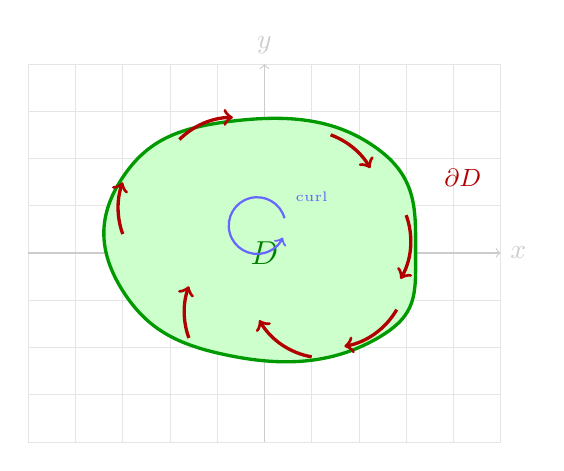
\begin{tikzpicture}[scale=1.2]
        % Grid background
        \draw[gray!20, very thin, step=0.5] (-2.5,-2) grid (2.5,2);
        \draw[gray!40, thin, ->] (-2.5,0) -- (2.5,0) node[right] {$x$};
        \draw[gray!40, thin, ->] (0,-2) -- (0,2) node[above] {$y$};

        % Region D with gradient fill effect
        \fill[green!20] plot[smooth cycle, tension=0.8] coordinates {(-1.5,0.8) (-0.3,1.4) (1.2,1.1) (1.6,0) (1.2,-0.9) (-0.3,-1.1) (-1.5,-0.4)};
        \draw[green!60!black, very thick] plot[smooth cycle, tension=0.8] coordinates {(-1.5,0.8) (-0.3,1.4) (1.2,1.1) (1.6,0) (1.2,-0.9) (-0.3,-1.1) (-1.5,-0.4)};

        % Region label
        \node[green!50!black, font=\large] at (0,0) {$D$};

        % Oriented boundary with multiple arrows
        \draw[->, red!70!black, very thick] (-0.9,1.2) arc (135:90:0.8);
        \draw[->, red!70!black, very thick] (0.7,1.25) arc (70:30:0.8);
        \draw[->, red!70!black, very thick] (1.5,0.4) arc (20:-30:0.8);
        \draw[->, red!70!black, very thick] (1.4,-0.6) arc (-30:-80:0.8);
        \draw[->, red!70!black, very thick] (0.5,-1.1) arc (-100:-150:0.8);
        \draw[->, red!70!black, very thick] (-0.8,-0.9) arc (-160:-200:0.8);
        \draw[->, red!70!black, very thick] (-1.5,0.2) arc (200:160:0.8);

        % Boundary label
        \node[red!70!black, font=\small] at (2.1,0.8) {$\partial D$};

        % Curl indicator in center
        \draw[->, blue!60, thick, rotate=15] (0.3,0.3) arc (0:320:0.3);
        \node[blue!60, font=\tiny] at (0.5,0.6) {curl};
    \end{tikzpicture}
\end{center}

\subsection{Classical Stokes' Theorem (Curl Theorem)}

For a surface $S \subset \mathbb{R}^3$ with boundary $\partial S$:
\[
    \iint_S (\nabla \times \mathbf{F}) \cdot d\mathbf{S} = \oint_{\partial S} \mathbf{F} \cdot d\mathbf{r}
\]

\begin{center}
    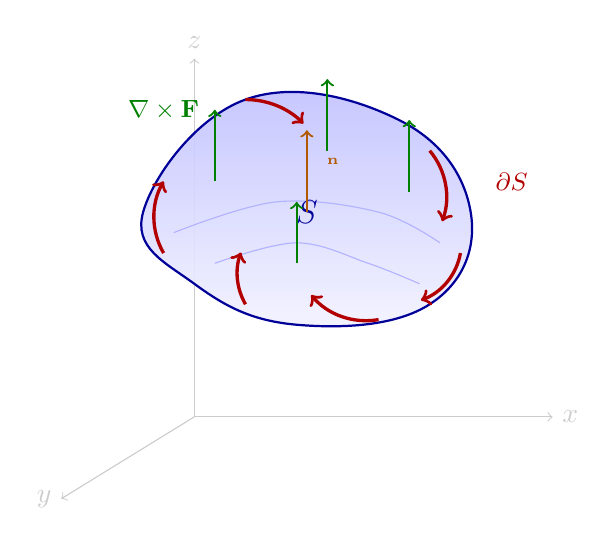
\begin{tikzpicture}[scale=1.3]
        % 3D axes hint
        \draw[gray!40, thin, ->] (-0.5,-1.5) -- (3,-1.5) node[right] {$x$};
        \draw[gray!40, thin, ->] (-0.5,-1.5) -- (-0.5,2) node[above] {$z$};
        \draw[gray!40, thin, ->] (-0.5,-1.5) -- (-1.8,-2.3) node[left] {$y$};

        % Surface S (curved membrane)
        \shade[top color=blue!25, bottom color=blue!5, opacity=0.9]
        plot[smooth cycle, tension=0.7] coordinates {(-1,0.5) (0,1.6) (1.5,1.4) (2.2,0.5) (1.8,-0.4) (0.5,-0.6) (-0.5,-0.2)};
        \draw[blue!60!black, thick]
        plot[smooth cycle, tension=0.7] coordinates {(-1,0.5) (0,1.6) (1.5,1.4) (2.2,0.5) (1.8,-0.4) (0.5,-0.6) (-0.5,-0.2)};

        % Surface mesh lines for 3D effect
        \draw[blue!30, thin] plot[smooth, tension=0.6] coordinates {(-0.7,0.3) (0.3,0.6) (1.3,0.5) (1.9,0.2)};
        \draw[blue!30, thin] plot[smooth, tension=0.6] coordinates {(-0.3,0) (0.5,0.2) (1.2,0) (1.7,-0.2)};

        % Surface label
        \node[blue!60!black, font=\large] at (0.6,0.5) {$S$};

        % Normal vectors (curl field)
        \draw[->, green!50!black, thick] (-0.3,0.8) -- (-0.3,1.5);
        \draw[->, green!50!black, thick] (0.8,1.1) -- (0.8,1.8);
        \draw[->, green!50!black, thick] (1.6,0.7) -- (1.6,1.4);
        \draw[->, green!50!black, thick] (0.5,0) -- (0.5,0.6);
        \node[green!50!black, font=\small] at (-0.8,1.5) {$\nabla \times \mathbf{F}$};

        % Oriented boundary curve with arrows
        \draw[red!70!black, very thick, ->] (0,1.6) arc (90:45:0.8);
        \draw[red!70!black, very thick, ->] (1.8,1.1) arc (40:-20:0.7);
        \draw[red!70!black, very thick, ->] (2.1,0.1) arc (-10:-70:0.6);
        \draw[red!70!black, very thick, ->] (1.3,-0.55) arc (-80:-140:0.7);
        \draw[red!70!black, very thick, ->] (0,-0.4) arc (-150:-200:0.6);
        \draw[red!70!black, very thick, ->] (-0.8,0.1) arc (210:150:0.7);

        % Boundary label
        \node[red!70!black, font=\small] at (2.6,0.8) {$\partial S$};

        % Right-hand rule indicator
        \draw[orange!70!black, thick, ->] (0.6,0.5) -- (0.6,1.3);
        \node[orange!70!black, font=\tiny, right] at (0.7,1.0) {$\mathbf{n}$};
    \end{tikzpicture}
\end{center}

\subsection{Divergence Theorem (Gauss's Theorem)}

For a solid region $V \subset \mathbb{R}^3$ with boundary $\partial V$:
\[
    \iiint_V (\nabla \cdot \mathbf{F})\,dV = \iint_{\partial V} \mathbf{F} \cdot d\mathbf{S}
\]

\begin{center}
    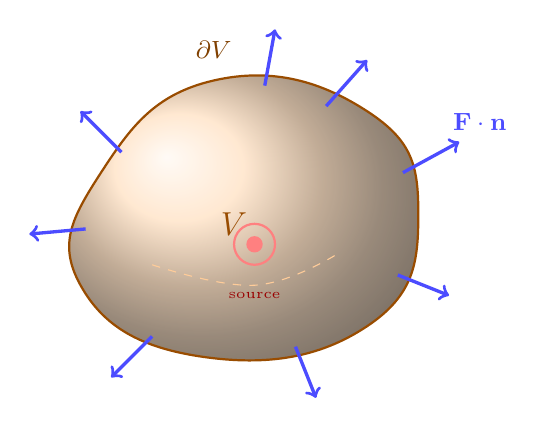
\begin{tikzpicture}[scale=1.3]
        % 3D blob (volume V) with shading
        \shade[ball color=orange!30, opacity=0.8]
        plot[smooth cycle, tension=0.8] coordinates {(-1.3,0.7) (-0.2,1.6) (1.3,1.3) (1.8,0.3) (1.3,-0.8) (-0.3,-1.1) (-1.5,-0.4)};
        \draw[orange!60!black, thick]
        plot[smooth cycle, tension=0.8] coordinates {(-1.3,0.7) (-0.2,1.6) (1.3,1.3) (1.8,0.3) (1.3,-0.8) (-0.3,-1.1) (-1.5,-0.4)};

        % Inner contour for 3D depth
        \draw[orange!40, dashed] plot[smooth, tension=0.7] coordinates {(-0.8,-0.2) (0.2,-0.4) (1.0,-0.1)};

        % Volume label
        \node[orange!60!black, font=\large] at (0,0.2) {$V$};

        % Outward flux arrows (vector field leaving surface)
        \draw[->, blue!70, very thick] (0.9,1.35) -- (1.3,1.8);
        \draw[->, blue!70, very thick] (1.65,0.7) -- (2.2,1.0);
        \draw[->, blue!70, very thick] (1.6,-0.3) -- (2.1,-0.5);
        \draw[->, blue!70, very thick] (0.6,-1.0) -- (0.8,-1.5);
        \draw[->, blue!70, very thick] (-0.8,-0.9) -- (-1.2,-1.3);
        \draw[->, blue!70, very thick] (-1.45,0.15) -- (-2.0,0.1);
        \draw[->, blue!70, very thick] (-1.1,0.9) -- (-1.5,1.3);
        \draw[->, blue!70, very thick] (0.3,1.55) -- (0.4,2.1);

        % Normal vector label
        \node[blue!70, font=\small] at (2.4,1.2) {$\mathbf{F} \cdot \mathbf{n}$};

        % Boundary surface label
        \node[orange!50!black, font=\small] at (-0.2,1.9) {$\partial V$};

        % Source/sink indicator inside
        \fill[red!50] (0.2,0) circle (0.08);
        \draw[red!50, thick] (0.2,0) circle (0.2);
        \node[red!60!black, font=\tiny] at (0.2,-0.5) {source};
    \end{tikzpicture}
\end{center}

\section{The Hodge Star Operator}

\begin{definition}[Hodge Star]
    On an oriented Riemannian $n$-manifold $(M, g)$, the \textbf{Hodge star operator} is a linear map:
    \[
        \star: \Omega^k(M) \to \Omega^{n-k}(M)
    \]
    satisfying $\alpha \wedge \star\beta = \langle \alpha, \beta \rangle \, \mathrm{vol}_g$ for $\alpha, \beta \in \Omega^k(M)$, where $\mathrm{vol}_g$ is the volume form.
\end{definition}

\begin{example}[Hodge Star on $\mathbb{R}^3$]
    With the standard metric and orientation:
    \begin{align*}
        \star 1  & = dx \wedge dy \wedge dz & \star(dx \wedge dy \wedge dz) & = 1  \\
        \star dx & = dy \wedge dz           & \star(dy \wedge dz)           & = dx \\
        \star dy & = dz \wedge dx           & \star(dz \wedge dx)           & = dy \\
        \star dz & = dx \wedge dy           & \star(dx \wedge dy)           & = dz
    \end{align*}
\end{example}

\begin{definition}[Codifferential]
    The \textbf{codifferential} $\delta: \Omega^k(M) \to \Omega^{k-1}(M)$ is defined by:
    \[
        \delta = (-1)^{n(k+1)+1} \star d \star
    \]
    On $\mathbb{R}^3$: $\delta = -\star d \star$ for appropriate degrees.
\end{definition}

\begin{proposition}[Divergence via Hodge Star]
    For a vector field $\mathbf{F}$ on $\mathbb{R}^3$:
    \[
        \nabla \cdot \mathbf{F} = \star d \star \mathbf{F}^\flat = \delta \mathbf{F}^\flat
    \]
    The divergence is the codifferential of the 1-form associated to $\mathbf{F}$.
\end{proposition}

\begin{definition}[Laplacian on Forms]
    The \textbf{Hodge Laplacian} (or Laplace-de Rham operator) is:
    \[
        \Delta = d\delta + \delta d = (d + \delta)^2
    \]
    On functions (0-forms) in $\mathbb{R}^n$, this recovers the usual Laplacian $\Delta f = \nabla^2 f$.
\end{definition}

\begin{center}
    \begin{tikzpicture}[scale=1]
        % Summary diagram
        \node[draw, rounded corners, fill=blue!10, minimum width=3cm, minimum height=1.5cm] (forms) at (0,0) {
            \begin{tabular}{c}
                Differential Forms \\
                $\Omega^k(M)$
            \end{tabular}
        };

        \node[draw, rounded corners, fill=green!10, minimum width=3cm, minimum height=1.5cm] (vec) at (6,0) {
            \begin{tabular}{c}
                Vector Calculus \\
                $\nabla, \nabla \times, \nabla \cdot$
            \end{tabular}
        };

        % Arrows
        \draw[->, thick] (forms) -- (vec) node[midway, above] {$\star$, metric};
        \draw[->, thick] (vec) -- (forms) node[midway, below] {unifies};

        % d and delta
        \draw[->, thick, red] (forms.north) to[out=90, in=90, looseness=1.5] node[above] {$d$} ($(forms.north)+(1.5,0)$);
        \draw[->, thick, blue] ($(forms.south)+(1.5,0)$) to[out=-90, in=-90, looseness=1.5] node[below] {$\delta = \star d \star$} (forms.south);
    \end{tikzpicture}
\end{center}

\begin{remark}[The Beauty of Differential Forms]
    The exterior derivative $d$ encapsulates:
    \begin{itemize}
        \item All differential operators (grad, curl, div) in a single operator
        \item All integral theorems in a single theorem ($\int_M d\omega = \int_{\partial M} \omega$)
        \item Topological invariants via de Rham cohomology ($d^2 = 0$)
    \end{itemize}
    The Hodge star $\star$ provides the missing link between the ``geometric'' exterior derivative and the ``metric-dependent'' operations like divergence and Laplacian.
\end{remark}

